\begin{slikaDesno}{fig/L_diode.pdf}
    \PID 
    У колу са слике познато jе $L = 100\unit{\upmu H}$ и 
    $V_{\rm G1} = V_{\rm G2} = 10\unit{V}$. Диода и
    прекидач су идеални. Прекидач се управља на основу тренутне вредности
    струjе калема. Када струjа калема достигне нулту вредност прекидач се
    затвара, а када струjа калема достигне вредност $I_0 = 1\unit{A}$ прекидач се
    отвара. У колу jе успостављен периодичан режим. 
    Одредити (а) струjу
    калема $i_L = i_L (t)$ и скцирати њен диjаграм. 
    (б) Одредити амплитудски спектар те струје, $|I_L [k]|$.    
\end{slikaDesno}

\REZULTAT 
(а) Тражена струја је периодична са основним периодом $Т_0 = 20\unit{\upmu s}$ на ком је дефинисана као 
$i_L = 1\unit{A} \tri\left(\dfrac{2t}{T_0}\right)$ што је приказано на слици \ref{fig:\ID.iL}. 
(б) Амплитудски спектар струје калема је 
$|I[k]| = \dfrac{1}{2}\unit{A} \sinc^2\left( \dfrac{k}{2} \right)$.

\begin{figure}
    \centering
    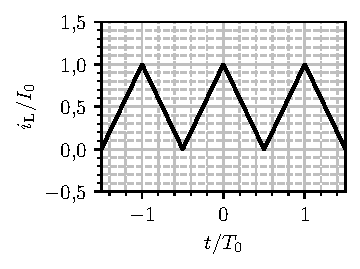
\includegraphics{fig/L_diode_iLL}
    \caption{Временски дијаграм струје калема}
    \label{fig:\ID.iL}
\end{figure}